\section{$\text{H}_2$/$\text{O}_2$ reaction kinetics: high-dimensional case}
\label{sec:app}

For the high-dimensional case, we aim to investigate the impact of the uncertain
pre-exponents ($A_i$'s) as well as the activation energies ($E_{a,i}$'s) on ignition 
delay during the H$_2$/O$_2$ reaction. The $A_i$'s are considered to be uniformly
distributed in the interval, $[0.9A_i^\ast, 1.1A_i^\ast]$. The $E_{a,i}$'s for all
reactions except $\mathcal{R}_6$ -- $\mathcal{R}_9$ and $\mathcal{R}_{13}$
are considered to be uncertain and uniformly distributed in the interval: 
$[0.99E_{a,i}^\ast, 1.01E_{a,i}^\ast]$. The nominal values, $A_i^\ast$ and $E_{a,i}^\ast$
corresponding to the different reaction rates are provided in~\cite{Yetter:1991}. 

The grad-free approach discussed earlier in~\ref{sub:gradfree} was used to compute the
active subspace. Using the iterative procedure, the convergence of the eigenvectors
was examined by tracking $\delta w_{1,j}^{(i)}$. In Figure~\ref{fig:conv_app} (left),
components of the converged eigenvector based on 50 samples using $\tau$ = 0.2 are plotted.
To illustrate convergence, we compare them with components of the eigenvector obtained
using 100 samples (twice as many). The variation of maximum $\delta w_{1,j}^{(i)}$ between
successive iterations during the course of the iterative procedure is illustrated in 
Figure~\ref{fig:conv_app} (right). 
%
\begin{figure}[htbp]
 \begin{center}
  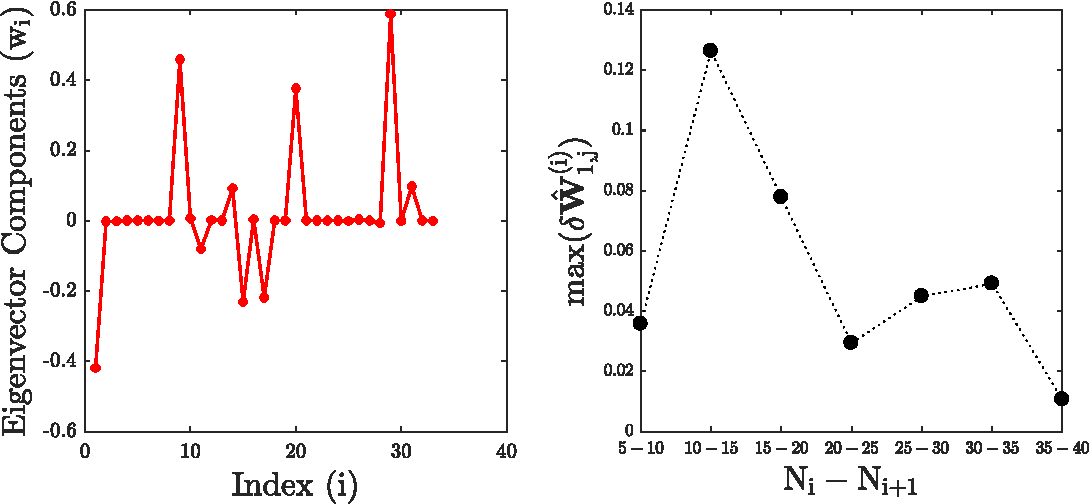
\includegraphics[width=0.8\textwidth]{./Figures/eigv10}
\caption{Left: An illustrative comparison of individual components of the converged dominant eigenvector obtained
using the two approaches discussed in~\ref{sub:grad} and~\ref{sub:gradfree}. Right: The quantity,  $\delta w_{1,j}^{(r)}$
is plotted for successive iterations to illustrate the convergence behavior.}
\label{fig:conv_app}
\end{center}
\end{figure}
%
  

